Let $p$ be an odd prime and let $E = Z( y^2 - x^3 - ax - b)$. We call $E$ an \textit{elliptic curve} defined over $\mathbb{F}_p$ if $4a^3 + 27b^2 \not\equiv 0 \text{ mod } p$. It was first realized by the mathematicians Abel and Jacobi in the 1700's that, remarkably, the points of $E$ (along with a special point $\OV$ called the point at infinity) can be made into a group using a very specific group operation. In this section we describe this group operation along with other algorithms needed for cryptographic purposes. 

\subsection{The Group Operation}  

Given two $\mathbb{F}_p$-rational points $P_1 = (x_1,y_1),P_2=(x_2,y_2)$ which we want to add together, we first define the value 
$$ s = 
\begin{cases}
\frac{y_1 - y_2}{x_1 - x_2} \text{ mod } p 	&\text{if } P_1 \neq P_2 \\
\frac{3x_1^2 - a}{2y_1} 	\text{ mod } p	&\text{if } P_1 = P_2 
\end{cases} 
$$ 
Then we define the coordinates of the point $P_3 = P_1 + P_2 $ to be 
\begin{align*}
	x_3 &= s^2 - (x_1 + x_2)  \\ 
	y_3 &=  s(x_3 - x_1) - y_1
\end{align*}
It's not immediately obvious that $P_3 = (x_3,y_3)$ is even a point on $E$ and less obvious that this operation satisfies the axioms of a group. The prrof of associativity is quite lenthy but we will at least show that the operation is closed in $E$. Let $u = x_1 + x_2$. We verify that $y_3^3 = x_3^3 + ax_3 + b$ mod $p$
\begin{align*}
	x_3^3 + ax_3 + b &= (s^2 - u)^3 +  a(s^2 - u) + b \\
	&= (s^4 - 2s^2u + u)(s^2 - u) + a(s^2 - u) + b \\
	&= s^6-s^4u-2s^4u+2s^2u^2+us^2-u^2 + a(s^2-u)+b \\
	&= s^6 - 3s^4u + s^2(2u^2 + u + a) - u^2 - au + b 					\\
	% &=  \\
	% &= s^6 -2s^4u + s^2u^2-2(s^4 - s^2u)x_1 + s^2x_1^2 - 2s^3y_1 -2suy_1 -2sx_1y_1 + y_1^2 \\
	&= s^2((s^4  -2s^2u + u^2)-2(s^2 - u)x_1 + x_1^2) - 2s^3y_1 -2suy_1 -2sx_1y_1 + y_1^2 \\
	&= s^2((s^2 - u)^2 -2(s^2 - u)x_1 + x_1^2) - 2s(s^3 -u - x_1)y_1 + y_1^2 \\
	&= s^2(x_3 - x_1)^2 - 2s(x_3 - x_1)y_1 + y_1^2 \\
	&= (s(x_3 - x_1) - y_1)^2  \\ 
	&= y_3^2 
\end{align*}
There is also a nice pictoral way to visualize the addition over the real number $\mathbb{R}$. Given points $P_1,P_2$, we calculate $P_3$ by finding the point of intersection of the line from $P_1$ to $P_2$ and $E$ and relecting it across the $x$ axis. 
\begin{center}
	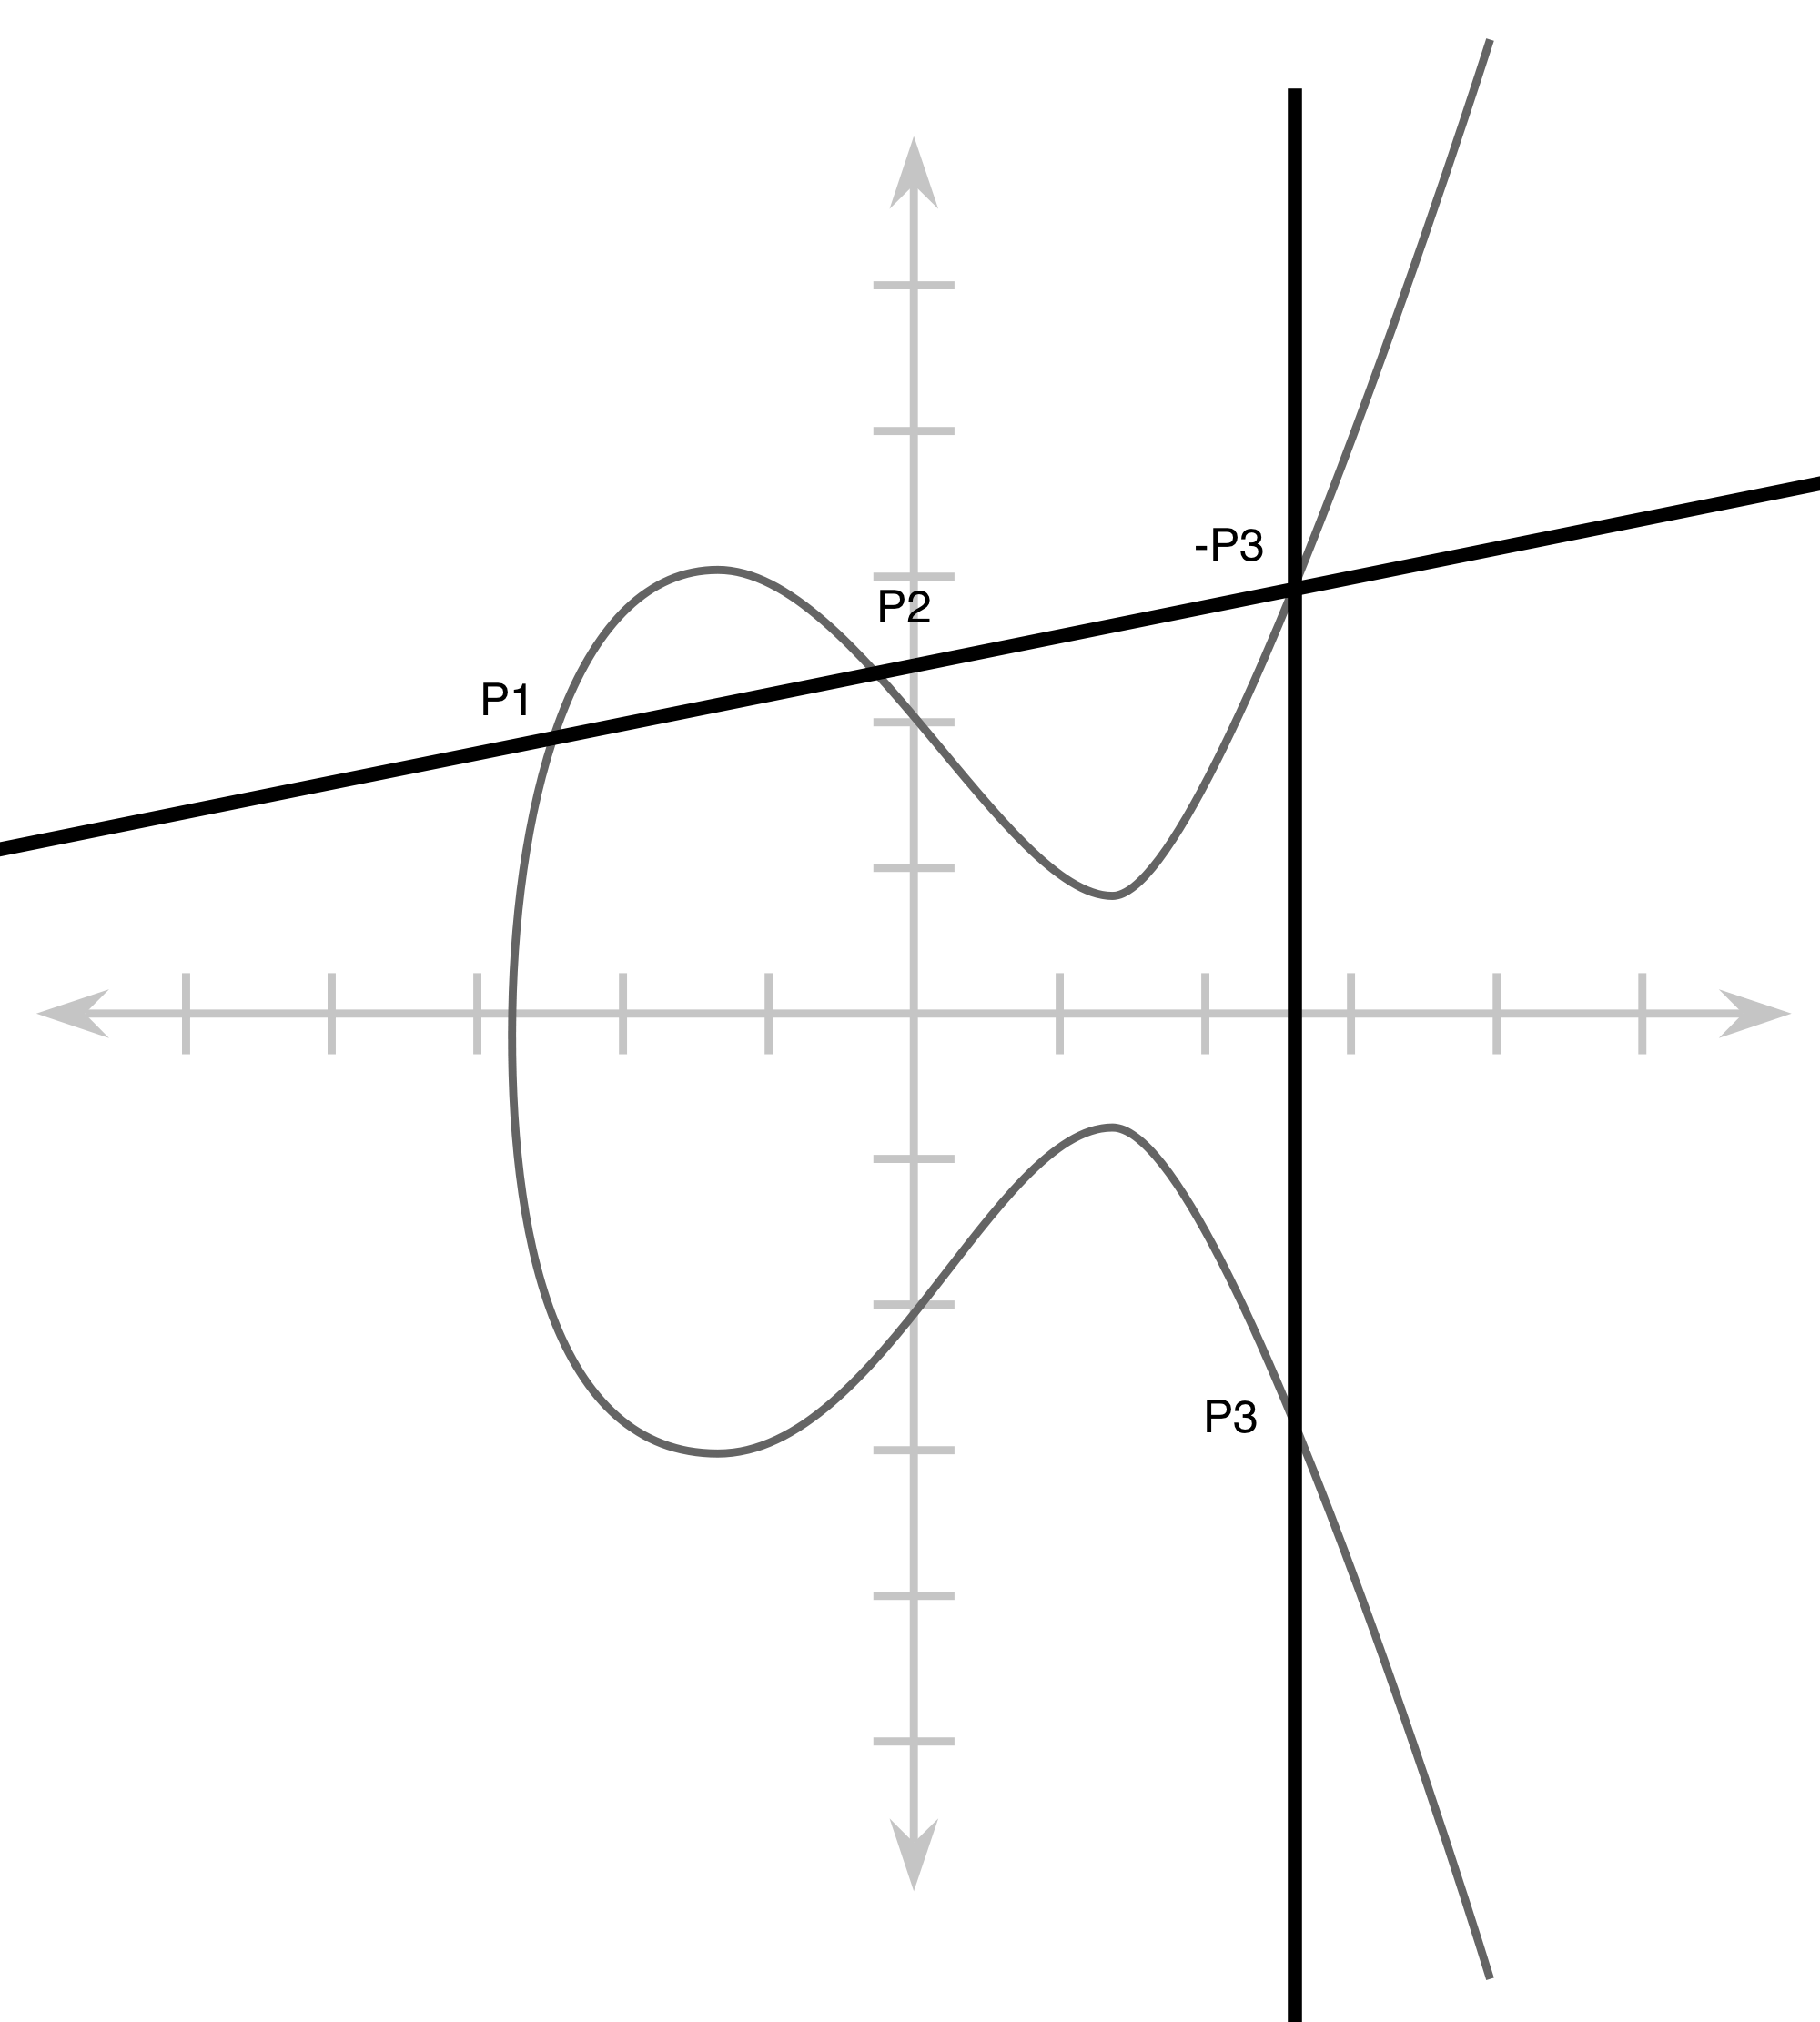
\includegraphics[width=10cm, height=7cm]{elliptic_curve_operation}
\end{center}
One may wonder about the inherent geometry of this curve, perhaps this may be exploited to compute the descrete logarithms in $E$. Towards this, it should be noted that the previous curve is defined over the real numbers. The picture changes quite drastically over fintite fields. For example, take $p$ to be the prime $3613$. Then the elliptic curve given by the equation $y^2 = x^3 + 2x + 3$ is graphed as 
\begin{center}
	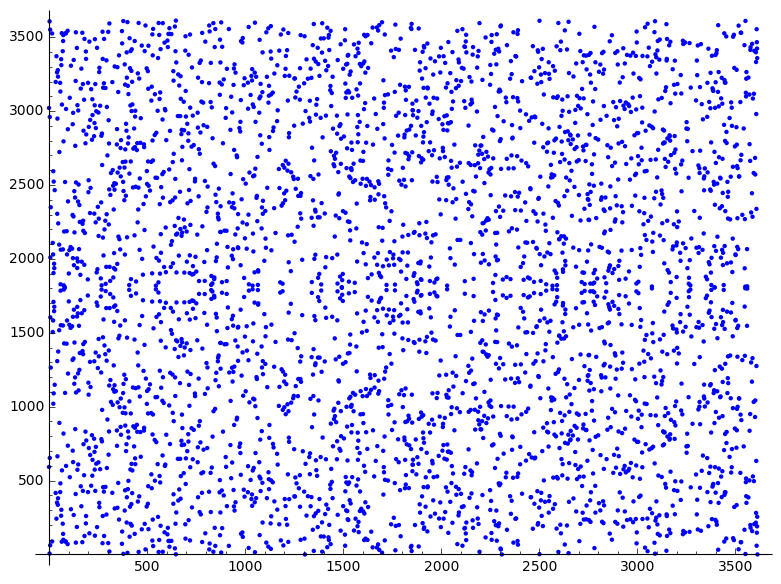
\includegraphics[width=9cm, height=7cm]{elliptic_finite}
\end{center}
So when the base field is finite, geometry is less apparent. The following algorithm describes how to add points on an elliptic curve.
\begin{algorithm} \label{ellipticlaw}
	\caption{The addition of two points $P_1 = (x_1,y_1),P_2 = (x_2,y_2)$ on an elliptic curve $E : y^2 + x^3 + ax + b$}
	\begin{algorithmic}[1]
		\Function{Add}{$E$,$P_1,P_2$}
			\If{$P_1 = \mathcal{O}$} 
				\State \Return{$P_2$}
			\ElsIf{$P_2 = \mathcal{O}$}
				\State \Return{$P_1$}
			\ElsIf{$P_1 = P_1$}
				\State $ s \leftarrow (3x_1^2 - a)(2y_1)^{-1} \text { mod } p $
		  	\Else
	  			\If{$x_1 \neq x_2$} 
	  				\State $ s \leftarrow (y_1 - y_2)(x_1 - x_2)^{-1} \text{ mod }p $
	  			\Else
	  				\State \Return{$\mathcal{O}$}
	  			\EndIf
	  		\EndIf 
	  		\State $ x_3 \leftarrow s^2 - x_1 -x_2 \text{ mod } p $
	  		\State $ y_3 \leftarrow  y_1 + s(x_3 - x_1) \text{ mod } p $ 
	  		\State \Return{$P_3 = (x_3,y_3)$}
	  	\EndFunction
	\end{algorithmic} 
\end{algorithm} 

Note that in steps $7$ and $10$, modular inverses must be calculated. Also note that if $x_1 = x_2$ but $P_1 \neq P_2$, then the second coordinates satisfy $y_1 = -y_2$. So the line from $P_1$ to $P_2$ is just a vertical line at $x_1$. This is taken to be the point at infinity $\mathcal{O}$. Also, when implementing this algorithm, the point at infinity $\mathcal{O}$ may be instantiated with any variable because no arithmetic is ever performed on it. 

\subsection{Scalar Multiplication of a Point}

For most discrete logarithm protocols (such as Diffie-Hellman or DSA), we require to add point $P$ to itself many times in order to perform discrete exponentiation. That is, given an integer $m$ we need to calculate $$[m]P = \overbrace{P + P + \cdots + P}^{m \text{ times}}$$ fast in order to be cryptographically reasonable. The following algorithm uses fast exponentiation by squaring in $E(\mathbb{F}_p)$ to achieve this. 


\begin{algorithm} 
	\caption{Scalar multiplication of a point $P$ by an integer $m$}
	\begin{algorithmic}[1]
		\Function{ScalarMult}{$m$,$P$}
		  	\If{$m =0$}
		  		\State \Return{$\mathcal{O}$}
		  	\ElsIf{$m=1$}
		  		\State \Return{$P$}
		  	\ElsIf{$m \equiv 0 \text{ mod } 2$}
		  		\State \Return{\Call{ScalarMult}{$m/2$,$P + P$}}
		  	\Else 
		  		\State \Return{$P$ + \Call{ScalarMult}{$m-1$,$P$}}
		  	\EndIf
	  	\EndFunction
	\end{algorithmic} 
\end{algorithm} 

\subsection{Finding Points}

Now that we have developed the arithmetic on an elliptic curve $E$, the next step is to find points on $E$. If $y^2 = x^3 + ax + b$ for $a,b \in \mathbb{F}_p$, then finding $\mathbb{F}_p$-rational points on $E$ is equivalent to determining if $x^3 + ax + b$ is a square mod $p$. This is a classical problem in number theory which can be reformulated to determing the value of the \textit{Legendre Symbol} of $a$ mod $p$, which is defined as 

$$ \lgr{a}{p} =
\begin{cases}
1 &\text{if }a \text{ is a square mod } p\\
-1 &\text{if }a \text{ is not a square mod }p\\
0 & \text{if } p \text{ divides }a
\end{cases} 
$$ 

where (in our case) $a = x^3 + ax + b$. The following five properties let us determine whether $a$ is a square mod $p$ in polynomial time. Let $a,b \in \mathbb{Z}$ and $p,q$ be odds primes.

\begin{enumerate}[(i)]
	\item \label{modequiv} If $a \equiv b$ mod $p$, then $\lgr{a}{p} = \lgr{b}{p}$
	\item \label{multiplicative} $\lgr{ab}{p} = \lgr{a}{p} \lgr{a}{p} $
	\item \label{1iseasy} $\lgr{-1}{p} = 1$ if $p \equiv 1 $ mod $4$, and $\lgr{-1}{p} = -1$ if $p \equiv 3 $ mod $4$
	\item \label{2iseasy} $\lgr{2}{p} = 1$ if $p \equiv \pm 1 $ mod $8$, and $\lgr{2}{p} = -1$ if $p \equiv \pm 3 $ mod $8$
	\item \label{reciprocity} If $p,q$ are distinct, then 
		$$ 
			\lgr{p}{q} = \lgr{q}{p} \text { if } p \text { or } q \equiv 1 \text{ mod } 4
		$$ 
		$$  
			\lgr{p}{q} = - \lgr{q}{p} \text { if } p \equiv q \equiv 3 \text{ mod } 4
		$$
\end{enumerate}

For example, to determine if $105$ is a square mod $227$, we simply compute 

\begin{align*}
	\lgr{105}{227} &\stackrel{\text{\eqref{multiplicative}}}{=} \lgr{3}{227}\lgr{5}{227}\lgr{7}{227} \\
	&\stackrel{\text{\eqref{reciprocity}}}{=} (-1) \lgr{227}{3}\lgr{227}{5} (-1) \lgr{227}{7} \\
	&\stackrel{\text{\eqref{modequiv}}}{=} \lgr{2}{3}\lgr{2}{5}\lgr{3}{7} \\
	&\stackrel{\text{\eqref{2iseasy}}}{=} (-1)(-1)(-1) \lgr{7}{3} \\
	&\stackrel{\text{\eqref{modequiv}}}{=} (-1) \lgr{1}{3} \\
	&= -1 
\end{align*}

So $105$ is a not a square mod $227$. The process of determining if an integer $a$ is a square mod $p$ is fairly quick but doesn't actually tell us the squareroot of $a$. If $\lgr{a}{p} = 1 $, then we may find $y$ such that $y^2 = a$ mod $p$ by breaking the calcultions into two cases: whether $p \equiv 3$ or $p \equiv 1$ mod 4. First, if $p \equiv 3 $ mod $4$, then $y = a^{(p+1)/4}$ satisfies $y^2 \equiv a $ mod $p$. The second case where $p \equiv 1 $ mod $4$ is more involved. Pick random $r$ such that $\lgr{r^2 - 4a}{p} =  -1 $ and write $d = r^2 - 4a$. let $\alpha = \frac{r+\sqrt{d}}{2}$ and $\alpha^{\frac{p+1}{2}} = \frac{y + v \sqrt{d}}{2}$ where $y,v$ are the coefficients of the elements $1$ and $\sqrt{d}$ in the $\frac{p+1}{2}$-th power expansion of $\alpha$. Then $y$ satisfies $y^2 \equiv a $ mod $p$. Putting all this together we obtain the following algorthm which finds random points on an elliptic curve $E$. 
\begin{algorithm} 
	\caption{Find random points on elliptic curve $E : y^2 - x^3 - ax - b$ modulo an odd prime $p$ }
	\begin{algorithmic}[1]
		\Function{RandomPoints}{$E$,$p$}
			\State $c \leftarrow x^3 + ax + b$ 
			\State pick random $x \in \lbrace 1, \dots , p-1 \rbrace $ with \Call{Legendre}{$c$,$p$} $= 1$ 
			\If{$p \equiv 3$ mod $4$}
				\State $y \leftarrow c^{(p+1)/4}$
			\Else
				\State pick random $x \in \lbrace 1, \dots , p-1 \rbrace $ with \Call{Legendre}{$r^2 - 4c$,$p$} $= - 1$
				\State $d \leftarrow r^2 - 4c, \alpha \leftarrow \frac{r+\sqrt{d}}{2}, y \leftarrow  \alpha^{\frac{p+1}{2}} - \frac{1}{2} v\sqrt{d}$
			\EndIf
			\State \Return $(x,y)$
	  	\EndFunction
	\end{algorithmic} 
\end{algorithm} 


\subsection{Counting Points}

When using an elliptic curve $E$ for discrete logarithm based cryptosystems, it is importance to know the number of points on $E$. This is because in 1978 Stephan Pohlig and Martin Hellman came up with an attack, described in [\ref{PohligHellman}], which uses the order of the group to solve discrete logs. The attack proceeds as follows: Given $G$, a finite cyclic group with order $N$, we may factor $N = p_1^{e_1}p_2^{e_2} \cdots p_s^{e_s}$ where $p_1,p_2,...,p_s$ are primes and $e_1,e_2,...,e_s \in \mathbb{Z}^+ $. All the subgroups $G_1,G_2,...,G_s$ of $G$ will have order $p_1^{e_1},p_2^{e_2},...,p_s^{e_s}$ respectively. Given an element $h = g^a \in G$, the Pohlig-Hellman attack solves for $a$ in the smaller subgroups $G_1,G_2,...,G_s$ and uses the Chinese remainder theorem to piece these solutions back together to solve for $a$ in the bigger group $G$. What they noticed is that when using this method, the complexity of solving for $a$ in $G$ (which can be done in $O(\sqrt{N})$ bit operations) gets reduced to $O(p_1^{e_1/2}) + O(p_2^{e_2/2}) + O(p_s^{e_s/2})$, i.e. the sum of the complexities of solving in the smaller groups. This means a group's bits of security is only as high as the bits of security of its largest subgroup. Therefore we want the order of the groups that we use to be prime, or at least a very small multiple of a prime, to avoid this attack. \\

With this is mind, we need an algorithm which calculates the number of points on an elliptic curve $E$ and thus the order of the group $E$. Intuitively, the number of points must be much less than $p^2$, for this would correspond to a curve that zeros every point in $\mathbb{Z}_p^2$. In fact, a much better estimate is given by Helmut Hasse. Denote the number of $\mathbb{F}_p$ rational points on $E$ by $\# E(\mathbb{F}_p)$, then  

\begin{equation}
	\# E(\mathbb{F}_p) = p + 1 + t
\end{equation}

where $|t| \leq 2  \sqrt{p}$. So essentially finding $\# E(\mathbb{F}_p)$ is equivalent to finding $t$. The first tractable algorithm to do so was designed by Rene Schoof in 1985 and was inspired by a very special map called \textit{the map of Frobeneous}
\begin{align*}
	\phi : E &\rightarrow E \\
	(x,y) &\mapsto (x^p,y^p)
\end{align*}
which happens to satisfy the equation 
\begin{equation} 
	\phi^2 + p = - t \phi \label{characteristic}
\end{equation} 
 in the endomorphism ring of $E$. That is, $\eqref{characteristic}$ is an equation of group homomorphisms from $E \rightarrow E$. The idea is to find $t$ in the interval $[-2 \sqrt{p},2 \sqrt{p}]$ which gives an equivalnce in \eqref{characteristic}. The problem is when $p$ is large ($300$ bits), this interval is just too big to brute force. Schoof's idea was to reduce this guess work by computing $t$ satisfying \eqref{characteristic} in the $l$-torsion subgroups $E[l] \subset E$ (the subgroup of all points $P$ satisfying $[l]P \equiv \OV$). Once this is done for a sufficient number of small primes $l$, the Chinese Remainder Theorem can be used to recover $t$. A detailed explanation of Schoof's algorithm can be found in algorithm \ref{schoof} in section \ref{algos}.

